\documentclass[a4paper]{article}
\usepackage[spanish]{babel}
\usepackage[utf8]{inputenc}
\usepackage{fancyhdr}
\usepackage{charter} % tipografia
%\usepackage{graphicx}
\usepackage[pdftex]{graphicx}
\usepackage{sidecap}
\usepackage{caption}
\usepackage{subcaption}
\usepackage{booktabs}
\usepackage{makeidx}
\usepackage{float}
\usepackage{amsmath, amsthm, amssymb}
\newtheorem{theorem}{Teorema}[section]
\newtheorem{corollary}{Corolario}[theorem]
\newtheorem{lemma}[theorem]{Lema}
\usepackage{amsfonts}
\usepackage{sectsty}
\usepackage{charter}
\usepackage{wrapfig}
\usepackage{listings}
\usepackage{hyperref} % links
\usepackage{algorithm} %http://www.ctan.org/pkg/algorithms
\usepackage{algorithmic}
\usepackage{color} % para snipets de codigo coloreados
\usepackage{fancybox} % para el sbox de los snipets de codigo
\definecolor{litegrey}{gray}{0.94}
% \newenvironment{sidebar}{%
% \begin{Sbox}\begin{minipage}{.85\textwidth}}%
% {\end{minipage}\end{Sbox}%
% \begin{center}\setlength{\fboxsep}{6pt}%
% \shadowbox{\TheSbox}\end{center}}
% \newenvironment{warning}{%
% \begin{Sbox}\begin{minipage}{.85\textwidth}\sffamily\lite\small\RaggedRight}%
% {\end{minipage}\end{Sbox}%
% \begin{center}\setlength{\fboxsep}{6pt}%
% \colorbox{litegrey}{\TheSbox}\end{center}}

%\newenvironment{codesnippet}{%
%\begin{Sbox}\begin{minipage}{\linewidth-2\fboxsep-2\fboxrule-4pt}\sffamily\small}%
%{\end{minipage}\end{Sbox}%
%\begin{center}%
%\colorbox{litegrey}{\TheSbox}\end{center}}

% \newenvironment{codesnippet}{\VerbatimEnvironment%
%   \noindent
%   %{\columnwidth-\leftmargin-\rightmargin-2\fboxsep-2\fboxrule-4pt}
%   \begin{Sbox}
%   \begin{minipage}{\linewidth-2\fboxsep-2\fboxrule-4pt}
%   \begin{Verbatim}
% }{%
%   \end{Verbatim}
%   \end{minipage}
%   \end{Sbox}%
%   \colorbox{litegrey}{\TheSbox}
% }

\newenvironment{codesnippet}{\VerbatimEnvironment%
  \noindent
  %      {\columnwidth-\leftmargin-\rightmargin-2\fboxsep-2\fboxrule-4pt}
  \begin{Sbox}
  \begin{minipage}{\linewidth}
  \begin{Verbatim}
}{%
  \end{Verbatim}
  \end{minipage}
  \end{Sbox}%
  \colorbox{litegrey}{\TheSbox}
}
\usepackage{fancyhdr}
\pagestyle{fancy}
%\renewcommand{\chaptermark}[1]{\markboth{#1}{}}
\renewcommand{\sectionmark}[1]{\markright{\thesection\ - #1}}
\fancyhf{}
\fancyhead[LO]{Sección \rightmark} % \thesection\
\fancyfoot[LO]{\small{Iv\'an Arcuschin, Mart\'in Jedwabny, Jos\'e Massigoge, Lucas Puterman}}
\fancyfoot[RO]{\thepage}
\renewcommand{\headrulewidth}{0.5pt}
\renewcommand{\footrulewidth}{0.5pt}
\setlength{\hoffset}{-0.8in}
\setlength{\textwidth}{16cm}
%\setlength{\hoffset}{-1.1cm}
%\setlength{\textwidth}{16cm}
\setlength{\headsep}{0.5cm}
\setlength{\textheight}{25cm}
\setlength{\voffset}{-0.7in}
\setlength{\headwidth}{\textwidth}
\setlength{\headheight}{13.1pt}
\renewcommand{\baselinestretch}{1.1} % line spacing
% \setcounter{secnumdepth}{2}
\usepackage{underscore}
\usepackage{caratula}
\usepackage{url}
\usepackage{enumitem}
\usepackage[usenames,dvipsnames]{xcolor}
\lstset{
    language=C++,
    basicstyle=\ttfamily,
    keywordstyle=\color{blue}\ttfamily,
    stringstyle=\color{red}\ttfamily,
    commentstyle=\color{ForestGreen}\ttfamily,
    morecomment=[l][\color{magenta}]{\#}
}
% ******************************************************** %
% TEMPLATE DE INFORME ORGA2 v0.1 %
% ******************************************************** %
% ******************************************************** %
% %
% ALGUNOS PAQUETES REQUERIDOS (EN UBUNTU): %
% ========================================
% %
% texlive-latex-base %
% texlive-latex-recommended %
% texlive-fonts-recommended %
% texlive-latex-extra? %
% texlive-lang-spanish (en ubuntu 13.10) %
% ******************************************************** %
\begin{document}
\thispagestyle{empty}
\materia{Algoritmos y Estructura de Datos III}
\submateria{Primer Cuatrimestre de 2015}
\titulo{Recuperatorio del Trabajo Práctico I}
%\subtitulo{Grupo: }
\integrante{Iv\'an Arcuschin}{678/13}{iarcuschin@gmail.com}
\integrante{Mart\'in Jedwabny}{885/13}{martiniedva@gmail.com}
\integrante{Jos\'e Massigoge}{954/12}{jmmassigoge@gmail.com}
\integrante{Lucas Puterman}{830/13}{lucasputerman@gmail.com}
\maketitle
% no footer on the first page
\thispagestyle{empty}
\newpage

\tableofcontents

\newpage
\section{Ejercicio 2 - Alta frecuencia}
\begin{figure}[h]
\begin{center}
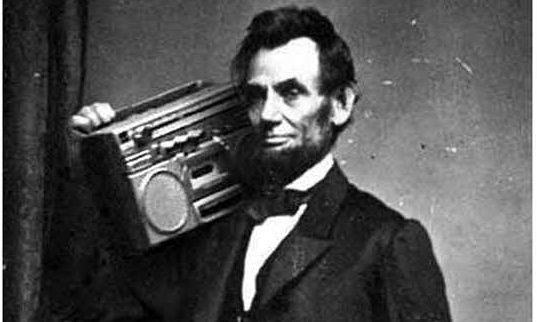
\includegraphics[width=0.6\textwidth] {imagenes/frecuencia.jpeg}
\end{center}
\end{figure}

\subsection{Problema a resolver}
Se tienen una lista de frecuencias que transmiten señales, donde cada una tiene un tiempo de inicio y fin y un costo por transmisión. El problema a resolver consiste en dar un algoritmo que minimice los costos, es decir, que para cada unidad de tiempo encuentre la frecuencia con menor costo e indique como ir cambiando de frecuencia acorde pasa el tiempo. A la vez, queremos transmitir todo el tiempo que sea posible.\\

\smallskip
Tenemos los siguientes parámetros de entrada:
	\begin{itemize}[noitemsep,nolistsep]
      \item $n$ = Cantidad de frecuencias
	  \item Luego vienen $n$ líneas con frecuencias, donde $F_{i}$ representa a la frecuencia en la línea $i$ con $1 \leq i \leq n$ y tiene los siguientes parámetros:
      \begin{itemize}
      \item $c_{i}$ = Costo de la frecuencia
      \item $b_{i}$ = Tiempo de inicio de la frecuencia
      \item $e_{i}$ = Tiempo de final de la frecuencia
      \end{itemize}
  	\end{itemize}
\smallskip

\begin{itemize}
\item Ejemplo: Situación inicial.

\begin{codesnippet}
2
10 1 16
5 6 10
\end{codesnippet}

Aquí se presentan dos señales, la primera tiene costo 10, inicio 1 y fin 16. La segunda tiene costo 5, inicio 6 y fin 10.

En este caso el algoritmo debe elegir la mejor señal para los tiempos 1 al 16.

En este ejemplo tenemos $n$ = 2 y luego $n$ señales:

\begin{table}[H]
\centering
\parbox{0.3\textwidth}{
    \begin{tabular}{ | l | l | l | l |}
    \hline
$F_{i}$ & $c_{i}$ & $b_{i}$ & $e_{i}$ \\ \hline
$F_{1}$ & 10 & 1 & 16 \\ \hline
$F_{2}$ & 5 & 6 & 10 \\ \hline
    \end{tabular}
}
\end{table}

\item Solución del ejemplo:

\begin{codesnippet}
130
1 1 6
2 6 10
1 10 16
\end{codesnippet}

La solución muestra que lo mejor es usar la primera señal de los tiempos 1 al 6, luego pasar a la segunda del 6 al 10 para, finalmente, retornar a la primer señal del 10 al 16.

El costo total de la transmisión anterior es 130 que es el menor costo posible para el ejemplo.

\end{itemize}

\subsection{Resolución planteada}

La solución planteada utiliza la técnica de \textit{Divide and Conquer}.
En este caso, se agregan todas las frecuencias recibidas a un vector y luego se llama a una función que se queda con dos problemas de menor complejidad en cada paso. Se llama a la misma recursivamente hasta llegar al caso base y luego se van uniendo las soluciones parciales hasta alcanzar un único vector con la solución final. \\


Veamos ahora como hacemos para unir dos soluciones parciales. En primer lugar, creo un indice de iteración para cada uno de los dos vectores que contienen los elementos que quiero unir (los llamamos vector izq y der):

\begin{codesnippet}
int izq_it <- 0
int der_it <- 0
\end{codesnippet}

Mientras ambos iteradores sean menores al tamaño del vector que itera, me fijo cual de los dos elementos a los que apuntan tiene menor principio y llamo a la función auxiliar $mergeAux$ que los irá agregando al resultado según corresponda. Es importante ver cual tiene menor principio porque queremos transmitir todo el tiempo posible.

\begin{codesnippet}
izq y der son Vector<Signal>
    donde Signal es tupla <numero:int, costo:int, principio:int, final:int>
Mientras izq_it < |izq| y der_it < |der| hacer:
    Si izq[izq_it].principio <= der[det_it].principio:
        mergeAux(izq, der, izq_it, der_it, result)
    Sino
        mergeAux(der, izq, der_it, izq_it, result)
    Fin if
Fin ciclo
\end{codesnippet}

Una vez que sale del ciclo, significa que al menos uno de los vectores fue recorrido completamente, por lo que nos queda agregar los elementos restantes del otro vector al vector solución:

\begin{codesnippet}
Mientras izq_it < |izq| hacer:
    result.agregarAlFinal(izq[izq_it])
    izq_it <- izq_it + 1
Fin ciclo

Mientras der_it < |der| hacer:
    result.agregarAlFinal(der[der_it])
    der_it <- der_it + 1
Fin ciclo
\end{codesnippet}

\vspace{1em}

Como vimos en el pseudocódigo arriba, la función auxiliar $mergeAux$ necesita comparar dos señales que pertencen una al vector $izq$ y la otra a $der$. Para hacer esto utiliza los iteradores pasados por parametro.\\

Pasamos a mostrar cómo la función auxiliar mergeAux compara dos señales dadas. Sean $F_{1}$ y $F_{2}$ las dos señales pertenecientes a $izq$ y $der$ apuntadas por los iteradores,  donde $b_{1} < b_{2}$. Sea también $resultado$ un vector que contendra frecuencias.\\

Al comparar las dos señales se nos presentan varios casos posibles:\\

\textit{Observacion:} Para todos los gráficos siguientes, las señales azules representan las de menor costo y las rojas las de mayor. Además, la que se encuentra más a la izquierda representa a $F_{1}$. \\
\\

\begin{itemize}
	\item Si $c_{1} \leq c_{2}$:
        \begin{itemize}
            \item Si $b_{2} \geq e_{1}$, entonces agrego $F_{1}$ a $resultado$ y aumento el iterador del vector al que pertenece $F_{1}$.
            \begin{figure}[H]
        		\centering
				\begin{subfigure}[b]{0.25\textwidth}
                	
\includegraphics[width=\textwidth]{imagenes/ej2-a.jpg}
                	\caption*{Lo llamaremos caso A}
        		\end{subfigure}%
			\end{figure}
            \item Si $b_{2} \leq e_{1} \land e_{1} < e_{2}$. Entonces, agrego $F_{1}$ a $resultado$, defino $b_{2} = e_{1}$ y aumento el iterador del vector al que pertenece $F_{1}$.

            \begin{figure}[H]
        	\centering
				\begin{subfigure}[b]{0.25\textwidth}
                	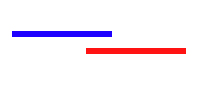
\includegraphics[width=\textwidth]{imagenes/ej2-b2.jpg}
                	\caption*{Lo llamaremos caso B}
        		\end{subfigure}%

				\begin{subfigure}[b]{0.25\textwidth}
                	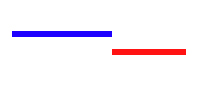
\includegraphics[width=\textwidth]{imagenes/ej2-b3c.jpg}
                	\caption*{$b_{2} = e_{1}$}
        		\end{subfigure}%
			\end{figure}
            \item Si $b_{2} \leq e_{1} \land e_{1} \geq e_{2}$. Entonces desestimo $F_{2}$, es decir, aumento el iterador del vector al que pertece $F_{2}$.
            \begin{figure}[H]
        		\centering
				\begin{subfigure}[b]{0.25\textwidth}
                	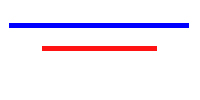
\includegraphics[width=\textwidth]{imagenes/ej2-c.jpg}
                	\caption*{Lo llamaremos caso C}
        		\end{subfigure}%
			\end{figure}
        \end{itemize}

	\item Si $c_{1} > c_{2}$:\\

\begin{itemize}
            \item Si $b_{2} \leq e_{1} \land e_{1} > e_{2}$. Entonces defino $F_{1}^{\prime} = F_{1}$ pero con $e_{1}^{\prime} = b_{2}$ y la agrego a $resultado$. Si $e_{2} < e_{1}$, entonces defino $b_{1} = e_{2}$ y no aumento ningún iterador.
            \begin{figure}[H]
        		\centering
				\begin{subfigure}[b]{0.25\textwidth}
                	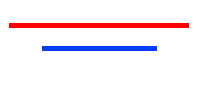
\includegraphics[width=\textwidth]{imagenes/ej2-c2.jpg}
                	\caption*{Lo llamaremos caso C$^{\prime}$}
        		\end{subfigure}%

				\begin{subfigure}[b]{0.25\textwidth}
                	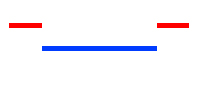
\includegraphics[width=\textwidth]{imagenes/ej2-c3.jpg}
                	\caption*{Aquí el primer segmento rojo es $F_{1}^{\prime}$ y el segundo $F_{1}$}
        		\end{subfigure}%
			\end{figure}

            \item Si $b_{2} \leq e_{1} \land e_{1} \leq e_{2}$. Entonces defino $e_{1} = b_{2}$ y agrego $F_{1}$ a $resultado$ y aumento el iterador del vector al que pertenece $F_{1}$.

            \begin{figure}[H]
        		\centering
				\begin{subfigure}[b]{0.25\textwidth}
                	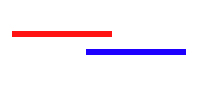
\includegraphics[width=\textwidth]{imagenes/ej2-b.jpg}
                	\caption*{Lo llamaremos caso B$^{\prime}$}
        		\end{subfigure}%

				\begin{subfigure}[b]{0.25\textwidth}
                	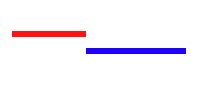
\includegraphics[width=\textwidth]{imagenes/ej2-b4c.jpg}
                	\caption*{$e_{1} = b_{2}$}
        		\end{subfigure}%
			\end{figure}

            \item Si $b_{2} \geq e_{1}$. Entonces agrego $F_{1}$ a $resultado$ y aumento el iterador del vector al que pertenece $F_{1}$.
            \begin{figure}[H]
        		\centering
				\begin{subfigure}[b]{0.25\textwidth}
                	
\includegraphics[width=\textwidth]{imagenes/ej2-a2.jpg}
                	\caption*{Lo llamaremos caso A$^{\prime}$}
        		\end{subfigure}%
			\end{figure}
        \end{itemize}

        Notemos que el único caso donde no se aumenta ninguno de los dos iteradores es el caso C$^{\prime}$. Sin embargo, como podemos ver en ese caso, luego de ejecutar ese llamado a $mergeAux$ nos queda nada más y nada menos que el caso A, y aumenta en uno nuestra cantidad de señales. \\ 
Por lo tanto al ejecutar un $merge$ entero con una entrada de tamaño $k$, donde $k$ es la suma de la cantidad de elementos de los dos vectores a unir, necesitamos a lo sumo $2k$ operaciones  Y se duplica la cantidad de señales retornadas, que es a lo sumo $2k$.\\ 

Por lo que podemos decir que $merge$ tiene complejidad lineal en la cantidad de elementos. \\

\end{itemize}

Ahora, veamos que si $n$ es la entrada del problema, el vector resultante luego de hacer el algoritmo tendrá a lo sumo tamaño $2n$
\begin{lemma}
Sea $n$ la cantidad de frecuencias recibidas al comienzo del problema. La cantidad de frecuencias resultantes al dar el menor costo de transmisión será a lo sumo $2n$.
\end{lemma}

\begin{proof}

Supongamos que puedo graficar en una línea de tiempo todos los $t$ que tienen comienzos y finales de las $n$ señales. De esta forma tendré $n$ comienzos y $n$ finales graficados a lo sumo porque dos señales pueden compartir los mismos comienzos o finales.\\

Por ejemplo:

            \begin{figure}[H]
        		\centering
				\begin{subfigure}[b]{0.5\textwidth}
azul                	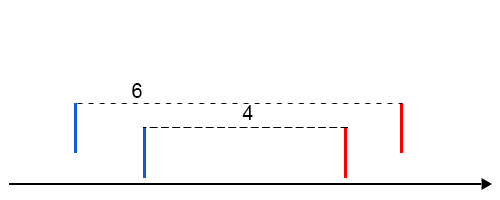
\includegraphics[width=\textwidth]{imagenes/demo1.jpg}
                	\caption*{Aqui podemos ver 2 frecuencias, por ende 2 comienzos (azul) y 2 finales (rojo)}
        		\end{subfigure}%
			\end{figure}

Como vimos arriba, solo se da en el caso C$^{\prime}$ que al comparar dos frecuencias me terminan quedando tres. Pero observemos que siempre que una frecuencia es separada en fragmentos, estos están delimitados por el comienzo o el final de otra frecuencia. Es decir, pondré como final de un fragmento el comienzo de otro, o pondré como comienzo de un fragmento el final de otro. \\

            \begin{figure}[H]
        		\centering
				\begin{subfigure}[b]{0.5\textwidth}
                	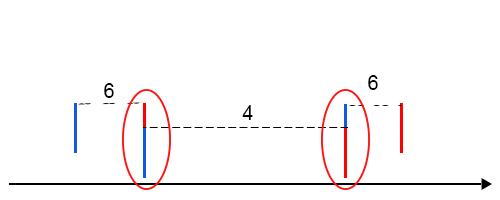
\includegraphics[width=\textwidth]{imagenes/demo2.jpg}
                	\caption*{Aqui podemos ver que aunque aumenta la cantidad de frecuencias, siguen usando los mismos comienzos y finales}
        		\end{subfigure}%
			\end{figure}


Pero como ya dijimos, en una entrada de tamaño $n$, tengo $n$ comienzos y $n$ finales. Entonces, la cantidad de veces que puedo cortar una frecuencia en dos está acotada por la cantidad de comienzos y finales que yo tenga, y estos son $2n$.
\end{proof}


%Por lo tanto, aunque una ejecución de $merge$ con un subproblema de tamaño $k$ con $k \leq n$ , donde $k$ es la suma de la cantidad de elementos de los dos vectores a unir, puede devolvernos $2k$ frecuencias, el tamaño total de la solución para todo el problema está acotado por $2n$.

Por lo tanto, aunque vimos que $merge$ puede retornar para una entrada $k$ algo de a lo sumo tamaño $2k$, donde $k$ es la suma de la cantidad de elementos de los dos vectores a unir. Uno puede pensar que cuando se ejecutan los $merge$ de nuestro algoritmo divide and conquer, se puede duplicar el tamaño de las frecuencias que devuelve en cada paso y aumentar de manera exponencial, esto es falso ya que estas están acotadas por $2n$.

\subsection{Complejidad propuesta}

Analizamos la complejidad usando Teorema Maestro\footnote{Thomas H. Cormen, Charles E. Leiserson, Ronald L. Rivest, and Clifford Stein. Introduction to Algorithms. The MIT Press, 2001.}:

Sean $a > 1$ y $b > 1$ constantes, sea $f(n)$ una función y sea
$T(n)$ definido en los enteros no negativos por la
recurrencia
$$T(n)= aT(\frac{n}{b}) + f(n)$$
$T(n)$ puede ser acotado asintóticamente de la siguiente manera: \\

1) Si $f(n) = \mathcal{O}(n^{\log_b a-\epsilon})$ para alguna constante $\epsilon > 0$, entonces, $T(n) = \Theta (n^{\log_b a})$. \\

2) Si $f(n) = \mathcal{O}(n^{\log_b a})$ entonces, $T(n) = \Theta (\log_b a  \log n )$. \\

3) Si $f(n) = \Omega (n^{\log_b a + \epsilon})$ para alguna constante $\epsilon > 0$ y si,
$af(\frac{n}{b}) \leq cf(n)$ para alguna constante $c < 1$ y todas las $n$ suficientemente grandes, entonces $T(n) = \Omega (f(n))$. \\

	% WAITTTTTT, no viste (en ningun lado lo dijiste) que el merge tiene complejidad lineal. Lo único que viste es que el tamaño total de la solución resultante está acotado por 2n. CUIDADO. ARREGLAR. WARNING.
	% OTRA COSA, quizas te creería más que las operaciones además del merge son constante si antes de esta demo de Complejidad hubiera un pseudocodigo, aunque se que era largo el pseudocodigo de este problema, fijate si le encontras alguna vuelta (no es tan importante esto que digo).
En cada paso nos quedamos con dos subproblemas que tienen la mitad de tamaño que el original, así que $a$ = 2 y $c$ = 2. Además de la recursión, se unen los resultados. Para esto llamamos a la función merge, que ya vimos que tiene complejidad lineal en la cantidad de elementos del arreglo. Más allá de esto, se hace una cantidad constante de comparaciones y asignaciones, por lo que podemos decir que $f(n)$  $\in$  $\Theta
(n)$. No podríamos usar el primer caso del teorema, porque $n^{\log_2 2-\epsilon}$ = $n^{1 - \epsilon}$ , y no es cierto que $f(n) \in$  $\Theta$ ($n^{1 - \epsilon}$ ). En cambio, podemos usar el segundo caso, porque como ya dijimos $f(n)$ $\in$ $\Theta (n)$ . Reemplazando, obtenemos $T(n)$ $\in$
 $\Theta$ ( $n^{\log_2 2}$  $log (n)$), o sea $T(n) \in$  $\Theta$ ($n$  $log (n)$).

\newpage
\subsection{Implementación en C++}
\lstinputlisting[language=C++]{codigo/ej2.cpp}

\subsection{Experimentación computacional}
La función que utilizamos para llevar a cabo las mediciones fue \texttt{std::clock}\footnote{Referencia \url{http://en.cppreference.com/w/cpp/chrono/c/clock}}. La unidad temporal que utilizamos para este ejercicio fue de nanosegundos.
La complejidad teórica calculada es de $\mathcal{O}(n*log(n))$

\subsubsection{Experimentación con instancias aleatorias}
Para generar las instancias aleatorias utilizamos la función \texttt{std::rand}\footnote{Referencia \url{http://en.cppreference.com/w/cpp/numeric/random/rand}} con determinados intervalos de valores para la variables, para obtener instancias coherentes. El detalle de intervalos es el siguiente:
\begin{itemize}
	\item Cantidad de muestras: 100
	\item Cantidad de frecuencias ($n$): de 1 a 3000
    \item Costos ($P$): 1 $\leq P \leq$ 10.000
	\item Para cada frecuencia, se verifico que su tiempo final fuera mayor que su inicio (no se usaron frecuencias invalidas).
\end{itemize}

Entonces, para cada $n$, del 1 al 3000 se generaron 100 instancias aleatorias de tamaño $n$.
Luego, estas fueron promediadas, arrojando los siguientes resultados:

\begin{figure}[H]
        \centering
        \begin{subfigure}[b]{0.5\textwidth}
                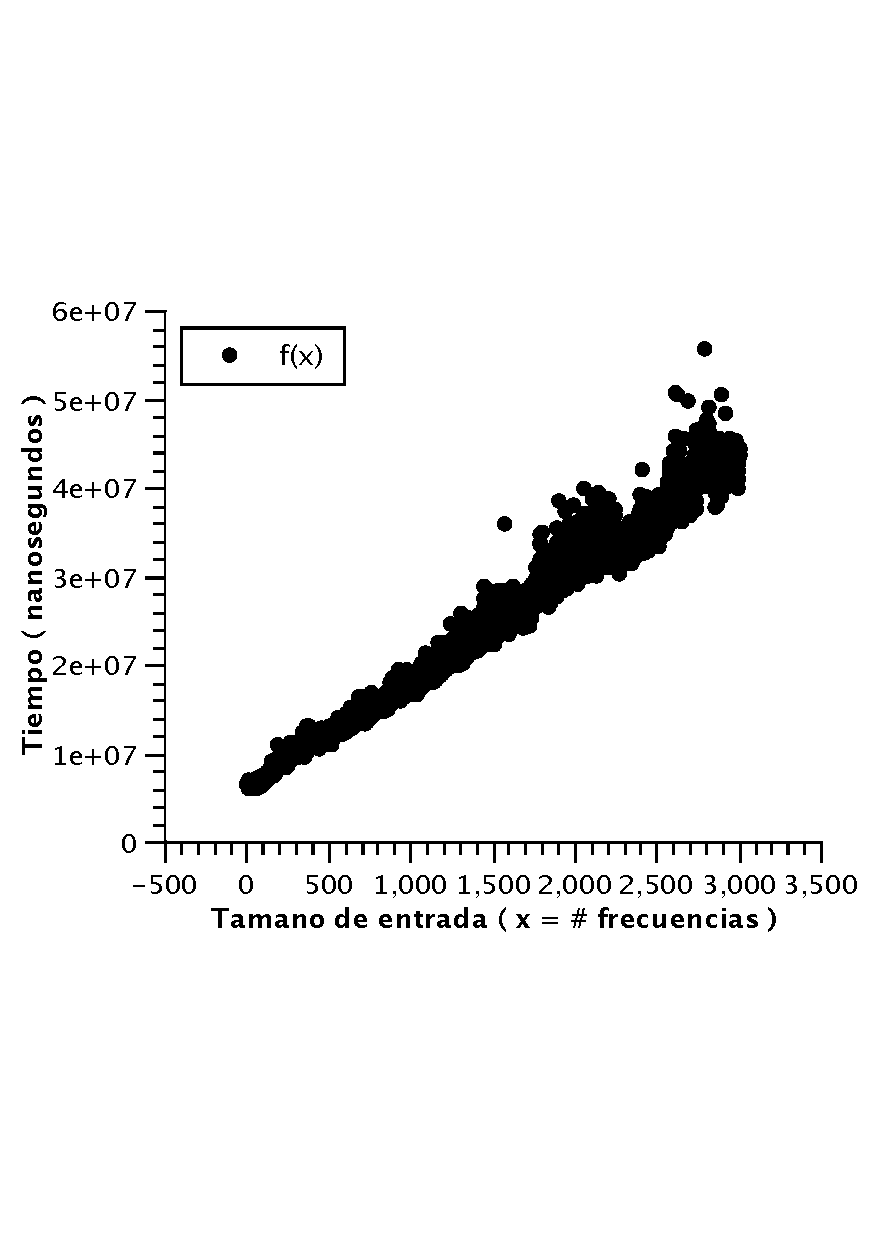
\includegraphics[width=\textwidth]{imagenes/af-rand-nlogn.pdf}
                \caption*{Tiempos sin procesar}
        \end{subfigure}%
\end{figure}

\begin{figure}[H]
        \centering
        \begin{subfigure}[b]{0.5\textwidth}
                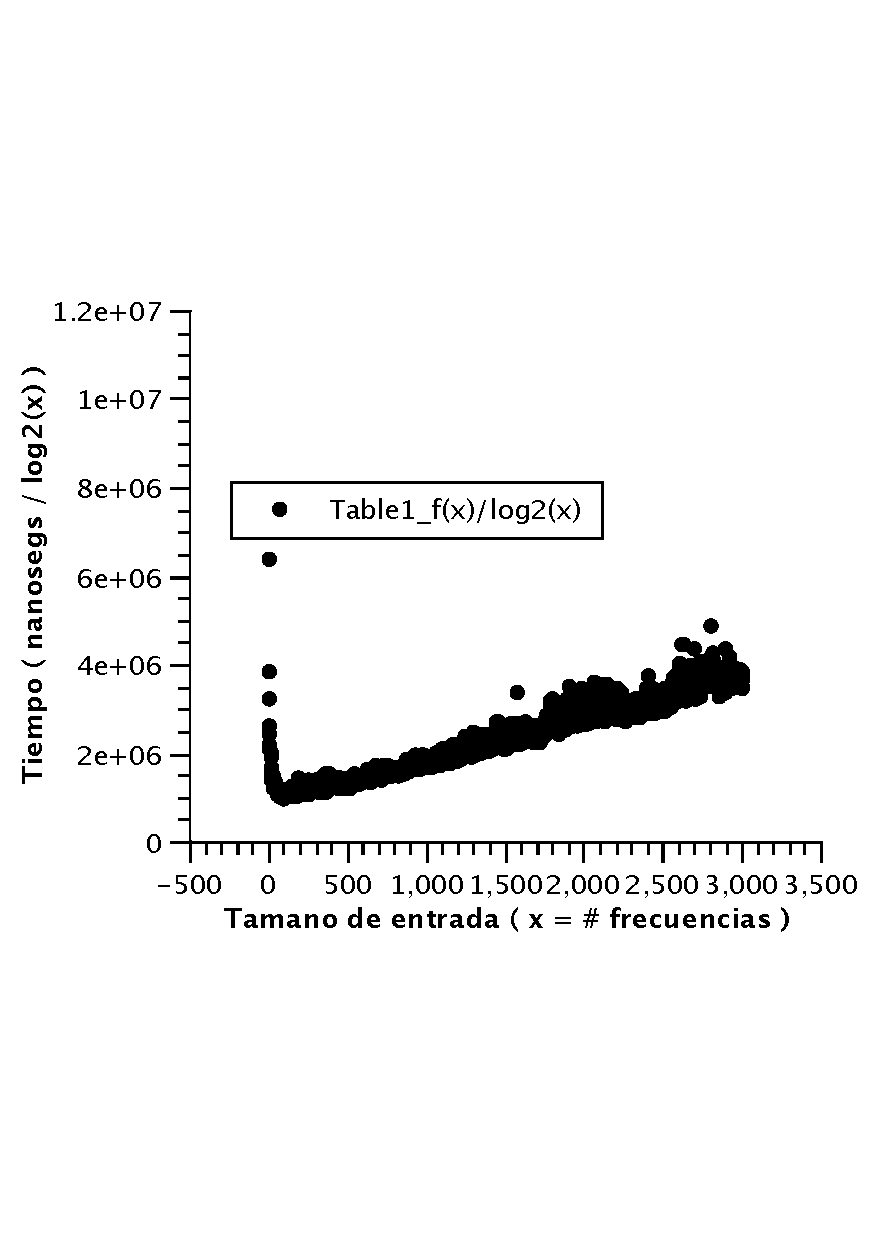
\includegraphics[width=\textwidth]{imagenes/af-rand-lineal.pdf}
                \caption*{Dividiendo a los tiempos por $\log(n)$}
        \end{subfigure}
\end{figure}

\begin{figure}[H]
        \centering
        \begin{subfigure}[b]{0.5\textwidth}
                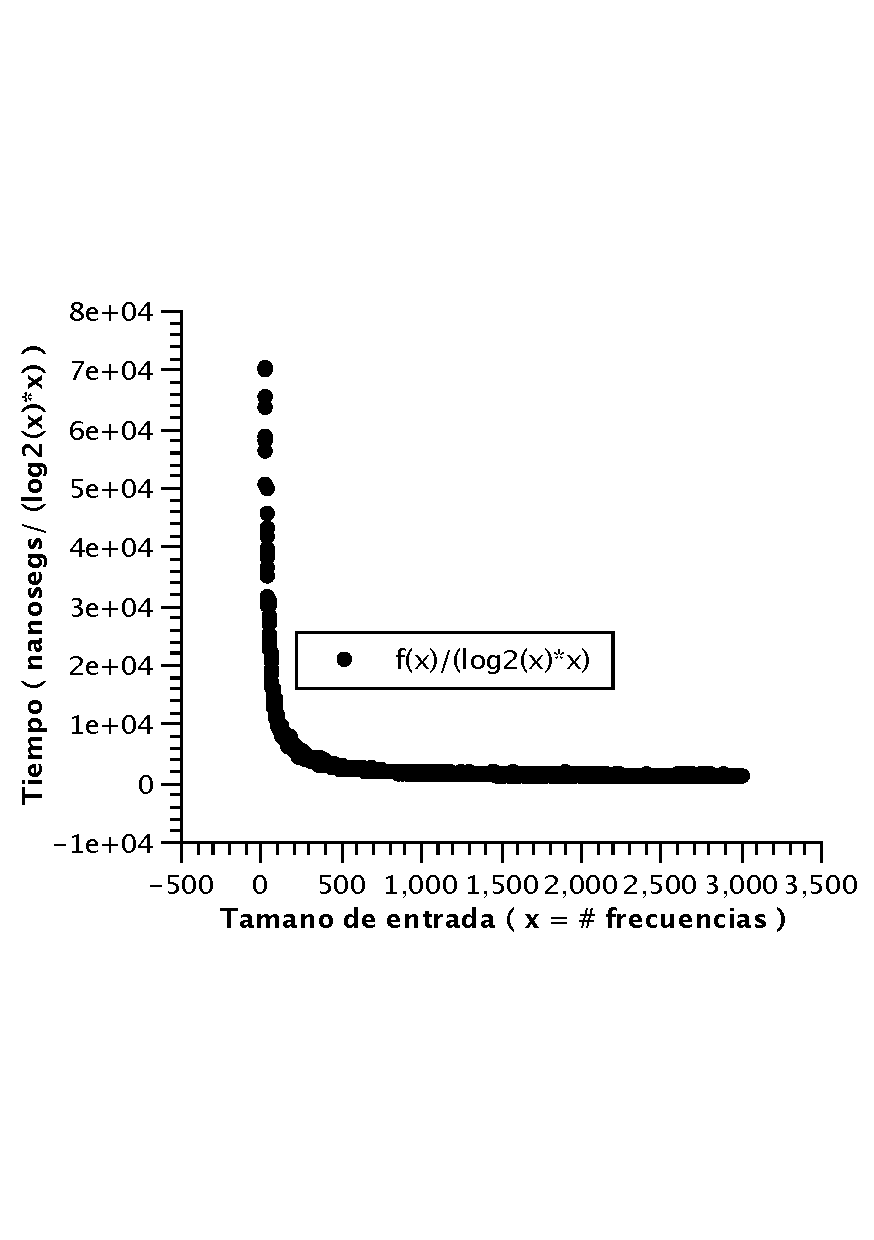
\includegraphics[width=\textwidth]{imagenes/af-rand-const.pdf}
                \caption*{Dividiendo a los tiempos por $n \log(n)$}
        \end{subfigure}
\end{figure}


A continuación, adjuntamos una tabla con los ultimos 20 valores obtenidos en este último paso, teniendo en cuenta que los casos fueron previamente ordenados segun el tamaño ($n$):

\begin{table}[H]
\parbox{0.3\textwidth}{
    \begin{tabular}{ | l | l | l | l |}
    \hline
Tamano($n$) & Tiempo($t$) & $t / log(n)$ & $t / n*log(n)$ \\ \hline
2,980 & 41,823,717 & 3,623,894.53913547 & 1,216.07199299848 \\ \hline
2,981 & 42,205,634 & 3,656,833.08407709 & 1,226.713547157695 \\ \hline
2,982 & 41,379,610 & 3,585,113.377975757 & 1,202.251300461354 \\ \hline
2,983 & 42,125,330 & 3,649,569.318887776 & 1,223.456023763921 \\ \hline
2,984 & 45,341,672 & 3,928,055.705472136 & 1,316.372555453129 \\ \hline
2,985 & 40,887,769 & 3,542,055.278169351 & 1,186.618183641324 \\ \hline
2,986 & 42,795,296 & 3,707,146.720857472 & 1,241.509283609334 \\ \hline
2,987 & 43,971,377 & 3,808,865.466588621 & 1,275.147461194717 \\ \hline
2,988 & 41,832,598 & 3,623,449.707752226 & 1,212.667238203556 \\ \hline
2,989 & 41,938,501 & 3,632,470.907368039 & 1,215.279661213797 \\ \hline
2,990 & 41,182,479 & 3,566,839.555032387 & 1,192.922928104477 \\ \hline
2,991 & 43,525,502 & 3,769,612.695656072 & 1,260.318520781034 \\ \hline
2,992 & 42,113,000 & 3,647,127.818332012 & 1,218.959832330218 \\ \hline
2,993 & 42,931,618 & 3,717,867.670108657 & 1,242.187661245792 \\ \hline
2,994 & 43,479,759 & 3,765,179.403366345 & 1,257.574951024163 \\ \hline
2,995 & 42,626,427 & 3,691,130.148415261 & 1,232.430767417449 \\ \hline
2,996 & 42,621,659 & 3,690,563.361166947 & 1,231.830227358794 \\ \hline
2,997 & 40,046,500 & 3,467,438.573756513 & 1,156.969827746584 \\ \hline
2,998 & 40,993,661 & 3,549,300.88989128 & 1,183.88955633465 \\ \hline
2,999 & 44,504,732 & 3,853,134.875349259 & 1,284.806560636632 \\ \hline
3,000 & 43,832,216 & 3,794,751.699991118 & 1,264.917233330373 \\ \hline
    \end{tabular}
}
\end{table}

A partir de la información suministrada, podemos observar que, en el primer gráfico las mediciones tienden a algo un poco más grande que lineal. Al dividir los tiempos por logaritmo de $n$ (segundo gráfico), se observa que tienden a ser algo lineal. Por último, en el último gráfico, se dividen además de por logaritmo de $n$, por $n$ y el gráfico que arroja es constante y mayor a 0. Por lo que podemos concluir que la complejidad de $\mathcal{O}(n*log(n))$ se condice con nuestra predicción de complejidad.

\subsubsection{Experimentación con instancias particulares}


Como quedo demostrado en la justificación de la complejidad teórica, el peor caso ocurre cuando al comparar dos frecuencias la de menor costo esta completamente contenida dentro de la de mayor costo. En este caso, la salida termina teniendo $2n-1$ señales. \\

\begin{figure}[H]
        		\centering
				\begin{subfigure}[b]{0.25\textwidth}
                	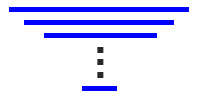
\includegraphics[width=\textwidth]{imagenes/ej2-wc-dibujo.jpg}
                	\caption{Aquí supongamos que cada señal tiene costo menor que la de arriba}
        		\end{subfigure}%
			\end{figure}

Generamos una muestra de peor caso de tamaños 1 a 3000 de la siguiente manera:
\begin{itemize}
	\item El costo de la primer frecuencia es 3001
	\item El comienzo de la primer frecuencia es 1
    \item El final de la primer frecuencia es 6001
    \item Cada frecuencia que se agrega disminuye en 1 el costo, aumenta en 1 el comienzo y disminuye en 1 el final
\end{itemize}



\begin{figure}[H]
        \centering
        \begin{subfigure}[b]{0.5\textwidth}
                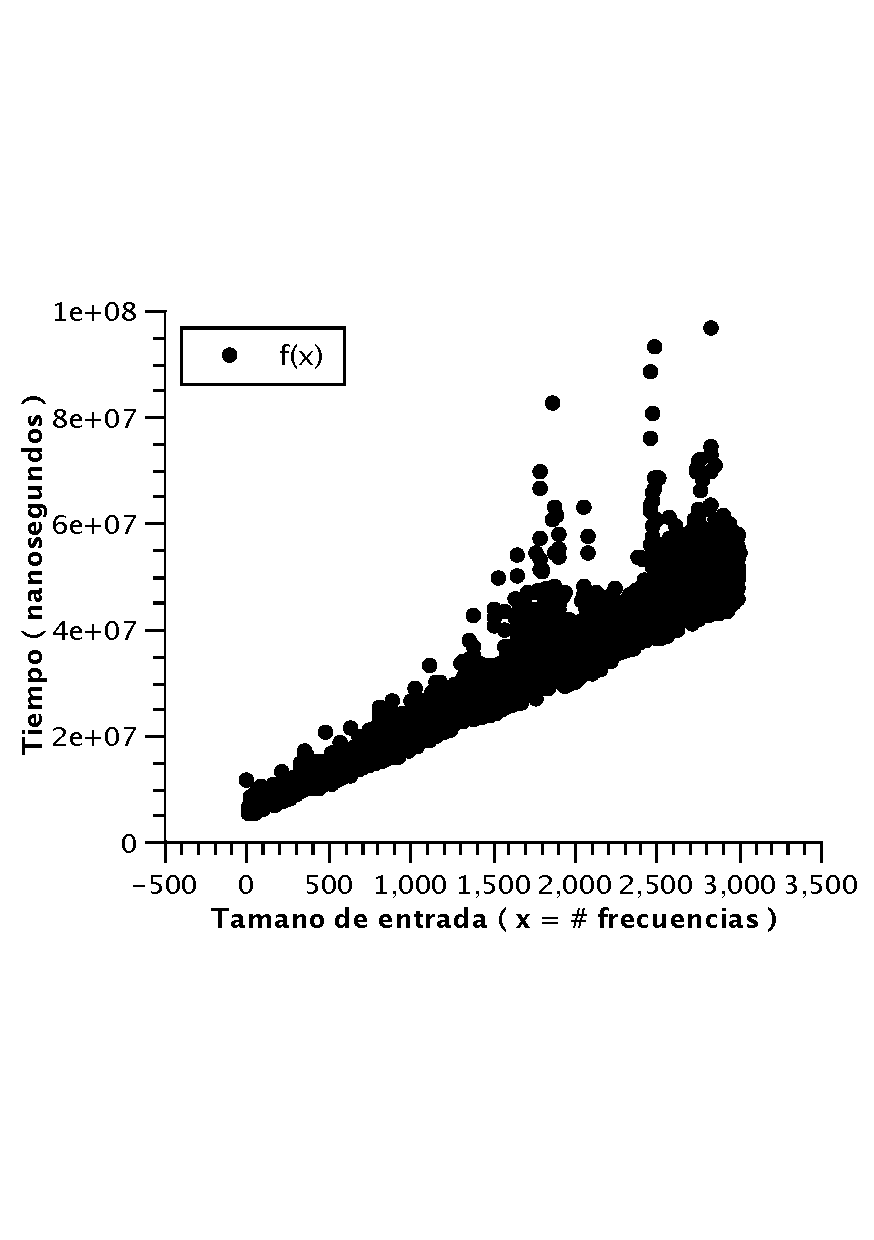
\includegraphics[width=\textwidth]{imagenes/af-wc-nlogn.pdf}
                \caption*{Tiempos sin procesar}
        \end{subfigure}%
\end{figure}

\begin{figure}[H]
        \centering
        \begin{subfigure}[b]{0.5\textwidth}
                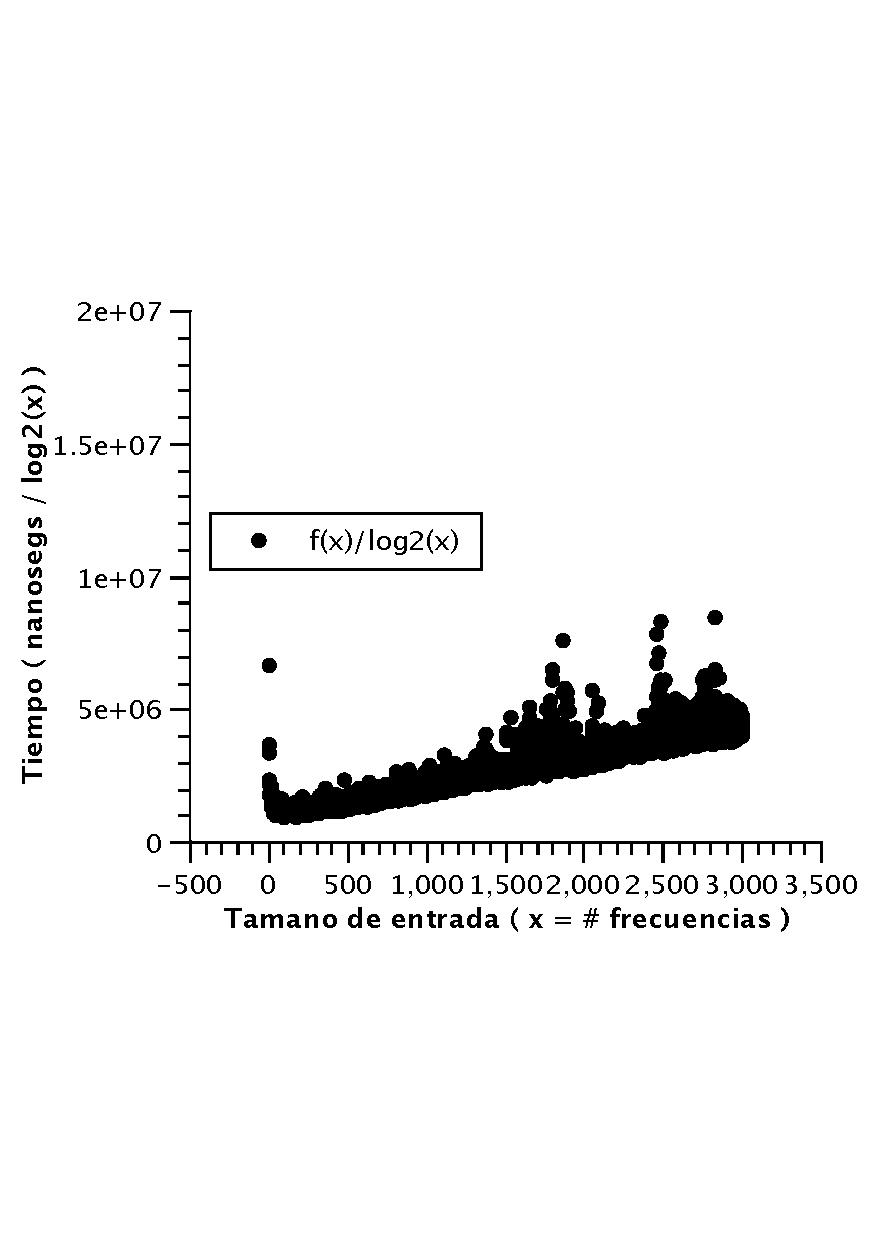
\includegraphics[width=\textwidth]{imagenes/af-wc-lineal.pdf}
                \caption*{Dividiendo a los tiempos por $\log(n)$}
        \end{subfigure}
\end{figure}

\begin{figure}[H]
        \centering
        \begin{subfigure}[b]{0.5\textwidth}
                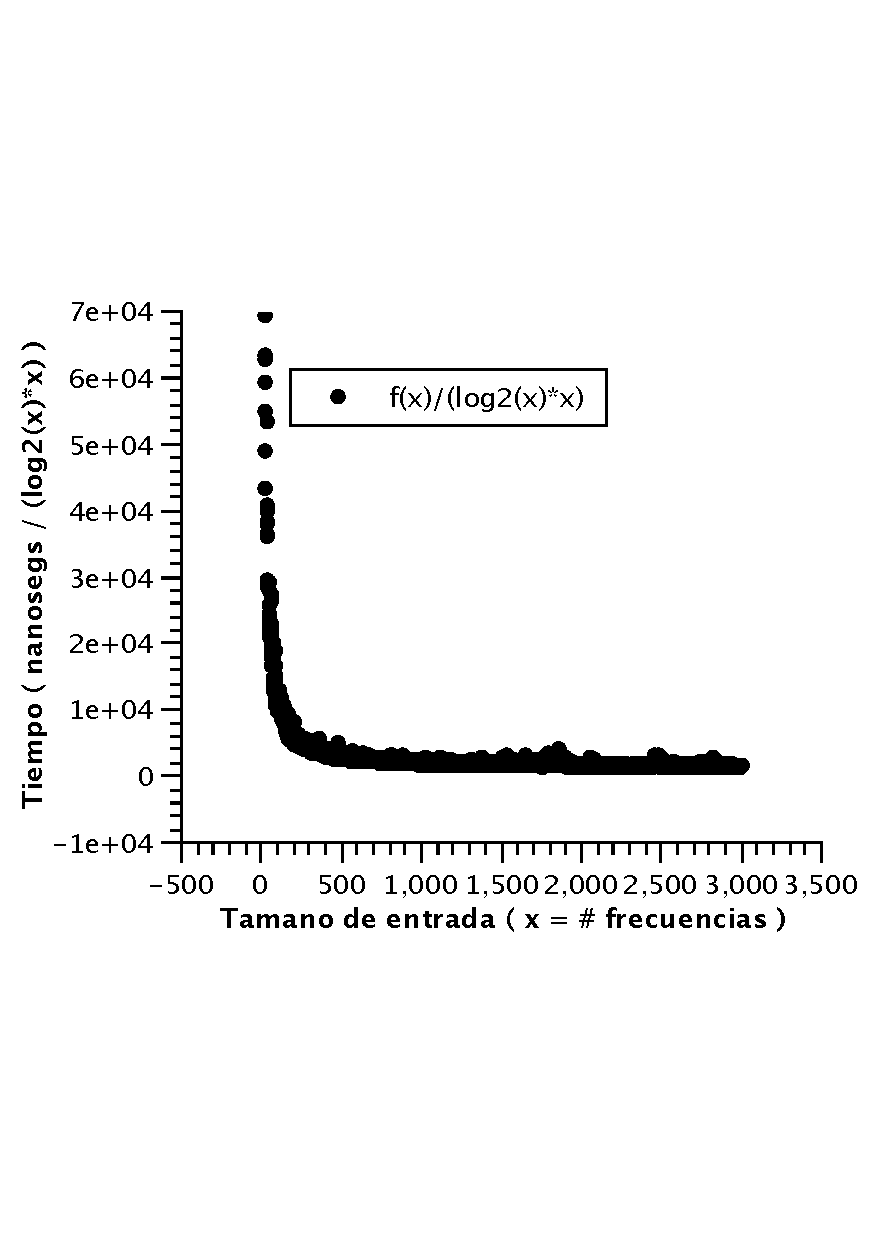
\includegraphics[width=\textwidth]{imagenes/af-wc-const.pdf}
                \caption*{Dividiendo a los tiempos por $n \log(n)$}
        \end{subfigure}
\end{figure}

A continuación, adjuntamos una tabla con los ultimos 20 valores obtenidos en este último paso, teniendo en cuenta que los casos fueron previamente ordenados segun el tamaño ($n$):

\begin{table}[H]
\parbox{0.3\textwidth}{
    \begin{tabular}{ | l | l | l | l |}
    \hline
Tamano($n$) & Tiempo($t$) & $t / log(n)$ & $t / n*log(n)$ \\ \hline
2,980 & 47,188,711 & 4,088,754.524179232 & 1,372.065276570212 \\ \hline
2,981 & 48,174,802 & 4,174,021.169127874 & 1,400.208376091202 \\ \hline
2,982 & 47,537,404 & 4,118,622.264314194 & 1,381.161054431319 \\ \hline
2,983 & 50,090,561 & 4,339,644.926021389 & 1,454.792130748035 \\ \hline
2,984 & 50,262,066 & 4,354,321.012249329 & 1,459.222859332885 \\ \hline
2,985 & 50,960,628 & 4,414,654.205912404 & 1,478.946132633971 \\ \hline
2,986 & 51,054,247 & 4,422,579.162716796 & 1,481.104876998257 \\ \hline
2,987 & 58,162,121 & 5,038,088.62161512 & 1,686.671784939779 \\ \hline
2,988 & 53,436,807 & 4,628,581.344801059 & 1,549.056674966887 \\ \hline
2,989 & 57,760,600 & 5,002,889.805053413 & 1,673.767080981403 \\ \hline
2,990 & 50,334,133 & 4,359,469.874376941 & 1,458.016680393625 \\ \hline
2,991 & 52,002,106 & 4,503,745.849466659 & 1,505.765914231581 \\ \hline
2,992 & 55,619,141 & 4,816,805.175903654 & 1,609.894778042665 \\ \hline
2,993 & 53,321,719 & 4,617,647.88796729 & 1,542.815866343899 \\ \hline
2,994 & 49,501,380 & 4,286,628.55316679 & 1,431.739663716362 \\ \hline
2,995 & 48,025,112 & 4,158,615.939924299 & 1,388.519512495592 \\ \hline
2,996 & 51,954,186 & 4,498,656.781775029 & 1,501.554333035724 \\ \hline
2,997 & 51,590,387 & 4,466,969.595815528 & 1,490.48034561746 \\ \hline
2,998 & 45,924,717 & 3,976,240.104930008 & 1,326.297566687795 \\ \hline
2,999 & 54,525,123 & 4,720,681.230346652 & 1,574.085105150601 \\ \hline
    \end{tabular}
}
\end{table}

A partir de la información suministrada, podemos observar que, en el primer gráfico las mediciones tienden a algo un poco más grande que lineal. Al dividir los tiempor por $\log(n)$ (segundo gráfico) se observa que el gráfico tiende a ser lineal. Por último, al dividir los tiempos por $n \log(n)$, el gráfico que arroja es constante y mayor a 0. Aunque este es peor caso, los gráficos siguen mostrando que se cumple la complejidad teórica calculada. Por lo que podemos concluir que la complejidad de $\mathcal{O}(n*log(n))$ se condice con nuestra predicción de complejidad.

\subsection{Adicionales}

Debido a un aumento en la demanda de nuestro servicio de transmisión de información, hemos duplicado
nuestro caudal de datos a transmitir y por tal motivo podemos ahora utilizar dos frecuencias en paralelo
en lugar de una sola. Quisiéramos resolver el mismo problema que antes pero ahora queremos transmitir
siempre que sea posible en dos frecuencias. En los momentos en que esto no sea posible, seguiremos
transmitiendo por una sola frecuencia, y obviamente en los momentos en los que esto último no se pueda
no transmitiremos nada. Es decir, el objetivo es transmitir información durante todo el tiempo que sea
posible y en la mayor cantidad de frecuencias en paralelo hasta un máximo de dos frecuencias, y hacer
esto invirtiendo la menor cantidad de dinero. Se pide desarrollar los siguientes puntos:

\begin{enumerate}
	\item \textit{Dar una idea de qué cambiaría en su algoritmo para resolver este nuevo problema.}

        Podríamos resolver este problema modificando el algoritmo que ya tenemos de la siguiente forma:

        Ejecutamos el algoritmo normalmente, pero guardando una copia extra del vector original que contiene a las señales, llamémosla $copia$.

        Una vez que se termina de ejecutar el algoritmo original, tendremos en el vector $resultado$ la opción de menor costo para la transmisión de las señales.

        Ahora, lo que se debe hacer es recorrer el vector $resultado$ y, por cada señal en $resultado$, buscar en el vector $copia$ la misma o el fragmento de la misma correspondiente y eliminarla.\\

        Esta tarea la haremos de la siguiente manera. Llamemos $R_{i}$ a la frecuencia en la posición $i$ de $resultado$. Buscamos en $copia$ la frecuencia correpondiente a $R_{i}$, llamemosla $C_{R_{i}}$. Actuaremos de la siguiente forma:

        Recordemos que dada una frecuencia $F_{i}$, $c_{i}$, $b_{i}$ y $e_{i}$ representan su costo, tiempo de comienzo y tiempo de fin respectivamente.
        \begin{itemize}

          \item Si $b_{i} = b_{R_{i}} \land e_{i} = e_{R_{i}}$ entonces esta señal se usa completamente, por lo que definimos $c_{R_{i}} = e_{R_{i}} = b_{R_{i}} = -1$.

          \item  Si $b_{i} > b_{R_{i}} \land e_{i} < e_{R_{i}}$ entonces me quedan dos fragmentos que no fueron usados, por lo que agrego al final de $copia$ una frecuencia $F$ con $c = c_{R_{i}}$, $b = b_{R_{i}}$ y $e = e_{i}$. Luego modifico a $C_{R_{i}}$ definiendole $b_{R_{i}} = b_{i}$.

          \item Si $b_{i} > b_{R_{i}} \land e_{i} = e_{R_{i}}$ o $b_{i} = b_{R_{i}} \land e_{i} < e_{R_{i}}$ entonces modifico $b_{R_{i}} = b_{i}$ o $e_{R_{i}} = e_{i}$ según sea necesario.

		\end{itemize}

		Una vez finalizado esto, podríamos tener frecuencias que tengan todos sus atributos en -1 (primer caso arriba), por lo que debemos crear otro vector, llamemoslo $v$ y lo llenaremos con los elementos de $copia$ que no tengan todo en -1. Luego, ejecutamos nuevamente el algoritmo de $mergeSort$ que usamos para resolver el ejercicio original sobre el vector $v$, obteniendo así las segundas mejores señales. \\

		\item \textit{¿Cómo afectaría este cambio en la complejidad temporal de su algoritmo?}

    Veamos: el agregado que le hacemos a nuestro algoritmo se divide en tres partes, una es crear el vector $copia$, la segunda es seleccionar las señales en $resultado$ y eliminar los fragmentos correspondientes en $copia$ y la tercera es volver a correr el algoritmo $mergeSort$ original sobre $copia$.

    Crear $copia$ no modifica nuestra complejidad temporal ya que lo hacemos al mismo tiempo que creamos el vector original.

    Sabemos que $resultado$ tiene tamaño de a lo sumo $2n-1$. Deberíamos recorrerlo entero y, por cada frecuencia, buscar el correspondiente en $copia$. Esto parece tener complejidad $\mathcal{O}(n^2)$. Sin embargo, podemos hacer algunos cambios en nuestra estructura para poder hacer esto de manera más eficiente.\\

    Actualmente tenemos la siguiente estructura $Signal$ en la implementación: \\

            \begin{codesnippet}
struct Signal {
    Signal() : numero(0), costo(0), principio(0), fin(0) {};
    Signal(const int n,const int c,const int p, const int f) : numero(n),
    costo(c), principio(p), fin(f) {};

    int numero;
    int costo;
    int principio;
    int fin;
};
\end{codesnippet}

	Notemos que estamos guardando el número de señal, que es ni más ni menos que el orden con que la señal fue guardada tanto en el vector original como en $copia$. Por esto, cada vez que ejecutando el algoritmo tengamos que buscar una señal de $resultado$ en $copia$, podemos hacerlo en $\mathcal{O}(1)$. Luego tenemos que modificarlo según sea necesario, esto lo hacemos también en $\mathcal{O}(1)$. Por lo que todo el proceso de recorrer $resultado$ y modificar $copia$ podemos hacerlo en $\mathcal{O}(2n) \in \mathcal{O}(n)$ porque vimos que $resultado$ tiene su tamaño acotado por $2n$. \\

   Ahora tenemos que crear el vector $v$ y llenarlo con las señales de $copia$ que cumplen las condiciones que vimos en el punto anterior. Esto esta acotado por el tamaño de $copia$ luego de modificarlo.

   Veamos cual es el tamaño de $copia$ viendo cuales son los tres casos posibles al comparar una señal de $resultado$ con una de copia:

           Llamemos $R_{i}$ a la frecuencia en la posición $i$ de resultado. Buscamos en $copia$ la frecuencia correpondiente a $R_{i}$, llamemosla $C_{R_{i}}$. Actuaremos de la siguiente forma: \\

        Recordemos que dada una frecuencia $F_{i}$, $c_{i}$, $b_{i}$ y $e_{i}$ representan su costo, tiempo de comienzo y tiempo de fin respectivamente.
        \begin{itemize}

          \item Si $b_{i} = b_{R_{i}} \land e_{i} = e_{R_{i}}$ entonces esta señal se usa completamente, por lo que definimos $c_{R_{i}} = e_{R_{i}} = b_{R_{i}} = -1$. \\

En este caso, el tamaño de $copia$ se mantiene igual, ya que no se agregan fragmentos. \\

          \item  Si $b_{i} > b_{R_{i}} \land e_{i} < e_{R_{i}}$ entonces me quedan dos fragmentos que no fueron usados, por lo que agrego al final de $copia$ una frecuencia $F$ con $c = c_{R_{i}}$, $b = b_{R_{i}}$ y $e = e_{i}$. Luego modifico a $C_{R_{i}}$ definiendole $b_{R_{i}} = b_{i}$. \\

En este caso, el tamaño de $copia$ aumenta en uno. \\
Recordemos que $resultado$ está ordenado cronologicamente por lo tanto mientras lo vaya recorriendo, cada frecuencia $R_{i}$ tendrá $b_{i} \geq e_{i-1}$. Entonces, al partir las frecuencias, la que agrego al final de $copia$ tiene que ser la que tenga el menor final ya que nunca volverá a ser buscada, mientras que la otra debe permanecer en su lugar, para que si tiene que volver a ser accedida en el futuro, esto se logre en $\mathcal{O}(1)$.\\ 


          \item Si $b_{i} > b_{R_{i}} \land e_{i} = e_{R_{i}}$ o $b_{i} = b_{R_{i}} \land e_{i} < e_{R_{i}}$ entonces modifico $b_{R_{i}} = b_{i}$ o $e_{R_{i}} = e_{i}$ según sea necesario. \\

          En este caso, el tamaño de $copia$ se mantiene igual, ya que no se agregan fragmentos. \\


\end{itemize}
Entonces, como podemos ver, el tamaño de $copia$ aumenta a lo sumo en uno por cada iteración. Esto se ejecuta tantas veces como elementos tenga $resultado$ y ya vimos que el tamaño de resultado está acotado por $2n$ por lo que $copia$ finaliza con a lo sumo $3n$ elementos. Por lo tanto, crear $v$ nos cuesta $\mathcal{O}(3n) \in \mathcal{O}(n)$\\

Por último, solo tenemos que correr nuestro $mergeSort$ con entrada $v$, como ya demostramos en el ejercicio original esto tiene complejidad $\mathcal{O}(n\log(n))$. Entonces con $v$ quedaría $\mathcal{O}(3n\log(3n)) \in \mathcal{O}(n\log(n))$. \\

Por lo tanto, no se modifica la complejidad del algoritmo, ya que esta termina siendo igualmente de:

$$\mathcal{O}(n\log(n))$$

\end{enumerate}


\subsection{Informe de modificaciones}
    \begin{itemize}
    \item Mejoras en descripción del problema.
    \item La resolución del problema fue modificada completamente.
    \item Aclaraciones sobre Teorema Maestro en la justificación de la complejidad.
    \item Aclaraciones sobre como fueron tomadas las muestras.
    \item Agregados los adicionales
\end{itemize}



\end{document}